\subsection*{Question 3.7}
We are to estimate the density of the second principal component. From
the figure \ref{fig:q37histograms} we see various histograms with
different numbers of bins. Our best guess is that around $12$ or $15$ bins
seems optimal. This depicts a mixture model with two modes. If we have
too small a number of bins, we lose the ability to capture the real
underlying distribution. On the other hand, if we choose too large a
number of bins, we end up with a very spiky histogram that is too
noisy to visualize the real distribution. Thus, one has to choose some
intermediate number of bins.

\begin{figure}[!htbp]
  \centering
  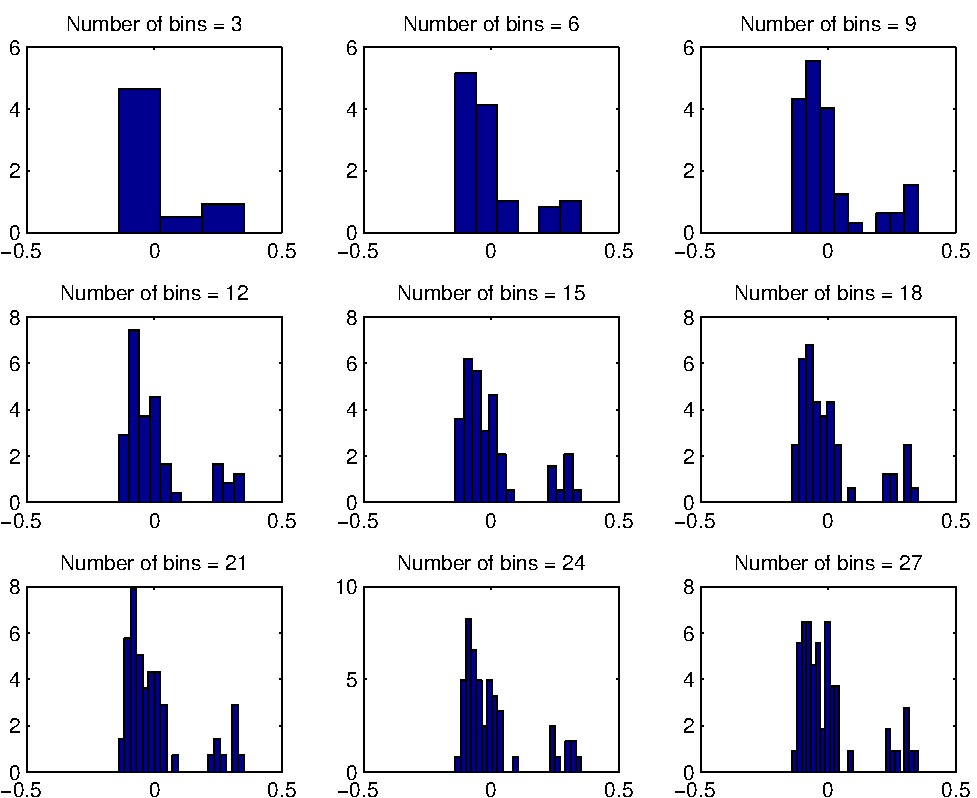
\includegraphics[width=0.85\textwidth]{./images/q37histograms}
  \caption{Shows histogram with various selections of bin numbers.}
  \label{fig:q37histograms}
\end{figure}

Next we are to try out kernel density estimator (kde), which can be
seen in figure \ref{fig:q37kde}. Again we see the same pattern as for
the histogram above. If we choose the bandwidth to be too low, it
results in a very spiky structure, while choosing the bandwidth to
large causes us to end up in the same situation as choosing a too small number
of bins: We lose the ability to capture the true form of the
underlying distribution. Somewhere between $0.03$ and $0.04$ seem to
be the optimal setting for capturing the two modes given by the second
principal component. Using automatic selection, the code gives the
optimal bandwidth $0.0329$ which is very close to our best guess. This
can be seen in figure \ref{fig:q37kdeauto}. It is easy to see that
when setting the bandwidth to $>0.05$, the two modes within the data
starts to merge into one.

\begin{figure}[!htbp]
  \centering
  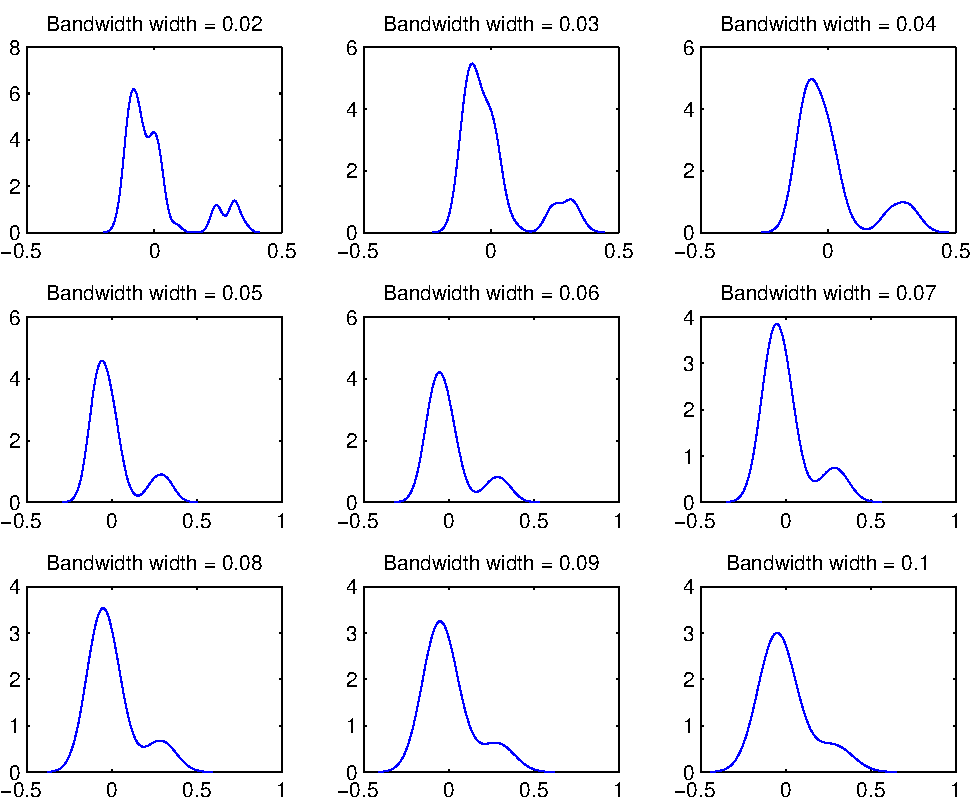
\includegraphics[width=0.85\textwidth]{./images/q37kde}
  \caption{Shows kernel density estimation for various selections of
    bandwidth.}
  \label{fig:q37kde}
\end{figure}

\begin{figure}[!htbp]
  \centering
  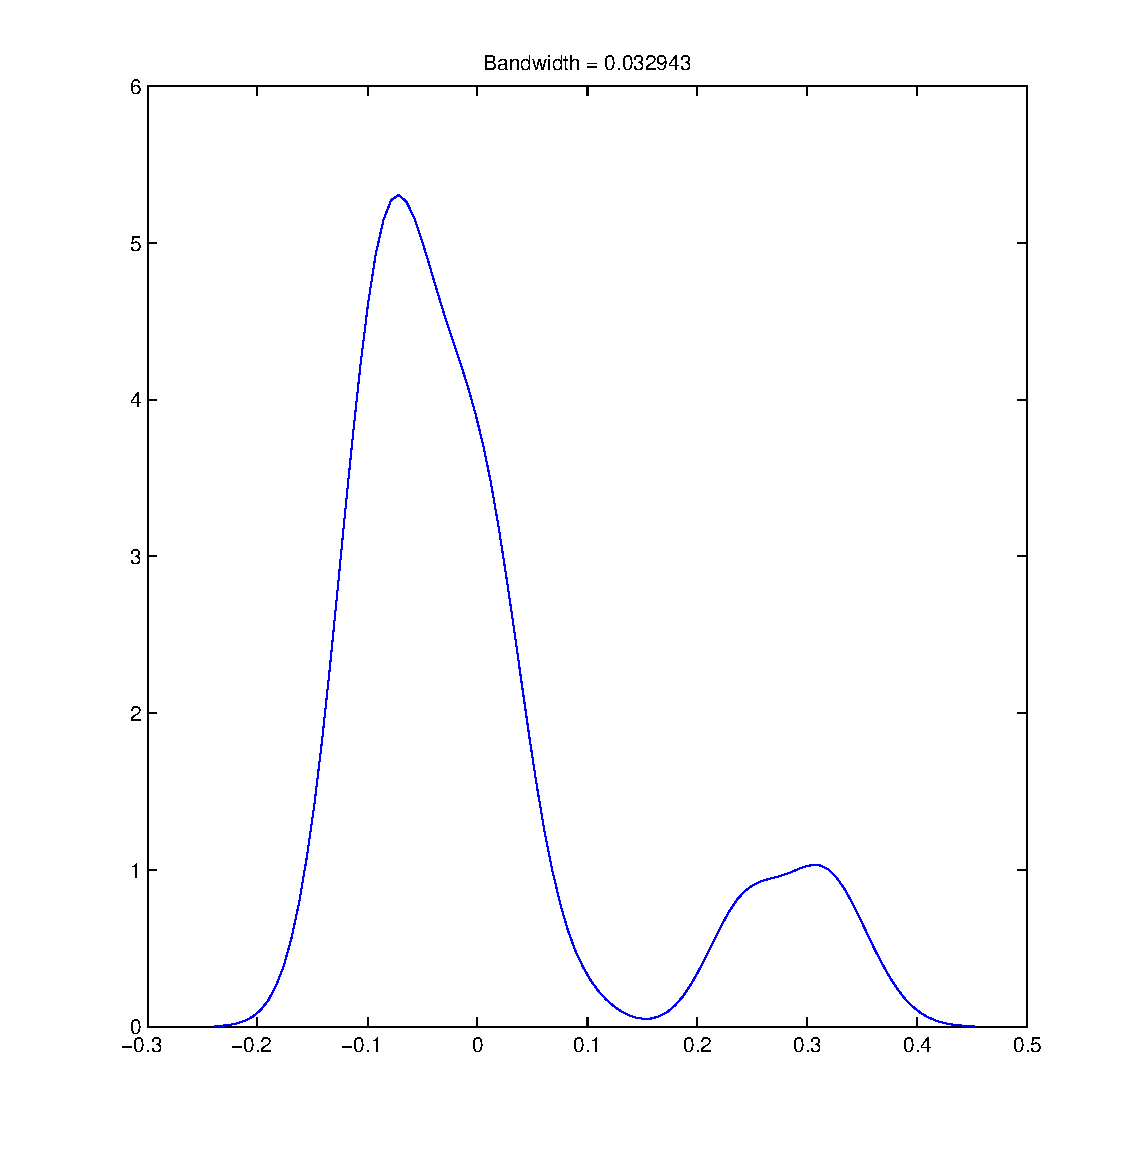
\includegraphics[width=0.65\textwidth]{./images/q37kdeauto}
  \caption{Shows kernel density estimation with automatic bandwidth
    selection.}
  \label{fig:q37kdeauto}
\end{figure}

\newpage

We are now to visualize $2d$ kernel density estimation based on the
first and second principal component. This is shown in figure
\ref{fig:q373dkde1} and \ref{fig:q373dkde2}. The figures shows the
same trends as the previously mentioned. Selecting the kernel
bandwidth too large causes the distribution to become too smooth,
thereby loosing the ability to capture the real form of the
distribution. Choosing the kernel bandwidth too small makes the
estimated distribution too spiky and noisy. So one has too choose some
intermediate. It has to be noted, that currently we select the same
bandwidth along both principal components. Better results can be
obtained by selecting individual bandwidth along the two different
axes.

\begin{figure}[!htbp]
  \centering
  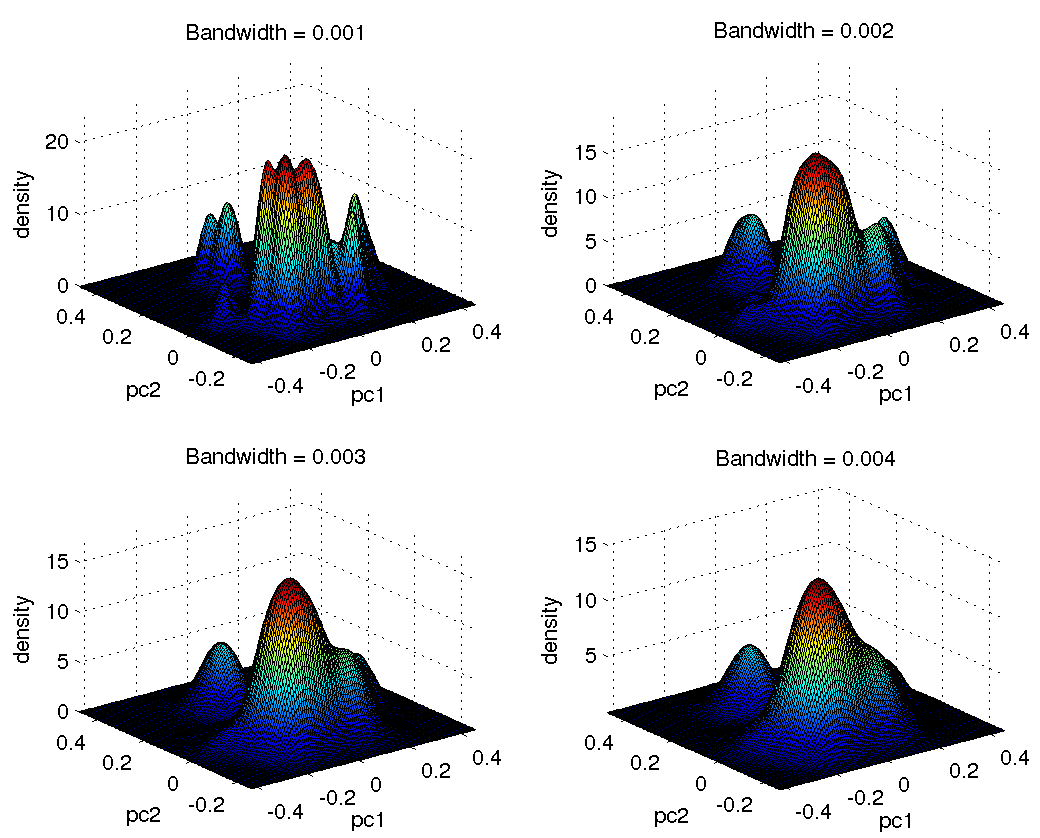
\includegraphics[width=1.0\textwidth]{./images/q373dkde1}
  \caption{Shows 2d kernel density estimations for various selections
    of bandwidth.}
  \label{fig:q373dkde1}
\end{figure}

\begin{figure}[!htbp]
  \centering
  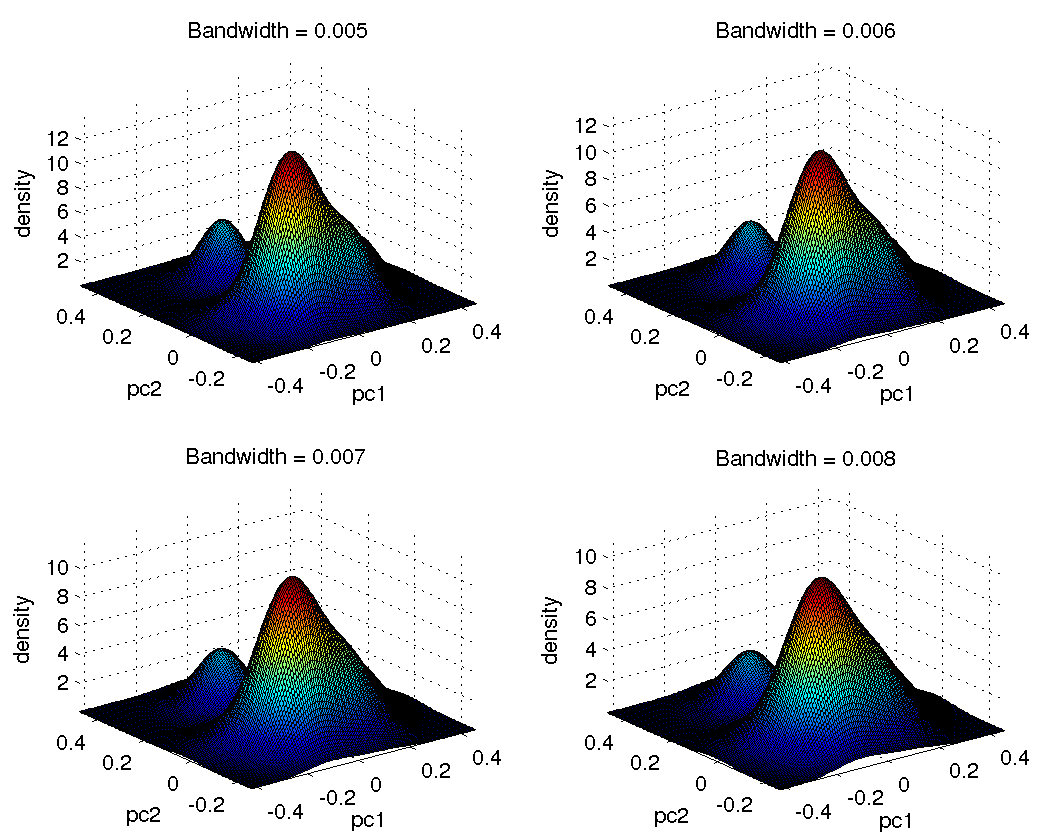
\includegraphics[width=1.0\textwidth]{./images/q373dkde2}
  \caption{Shows 2d kernel density estimations for various selections
    of bandwidth.}
  \label{fig:q373dkde2}
\end{figure}

\newpage

We are now to try out making density estimation using gaussian mixture
model with various numbers of components. This is shown in figure
\ref{fig:q37mog}. When using two components, we are only able to
capture two of the modes within the two principal components. Using
three, the result looks very reasonable, and this is our best guess at
the optimal value. Using four components, we start to get $\delta$-spikes
where the component collapses onto a data point. This can be seen
around pc1 $= 0.2$ and pc2 $= 0.0$. The problem is even more visible
when using five components. We see that the 'top' of the density is
now around $60$ as opposed to $25$ when using three components.

\begin{figure}[!htbp]
  \centering
  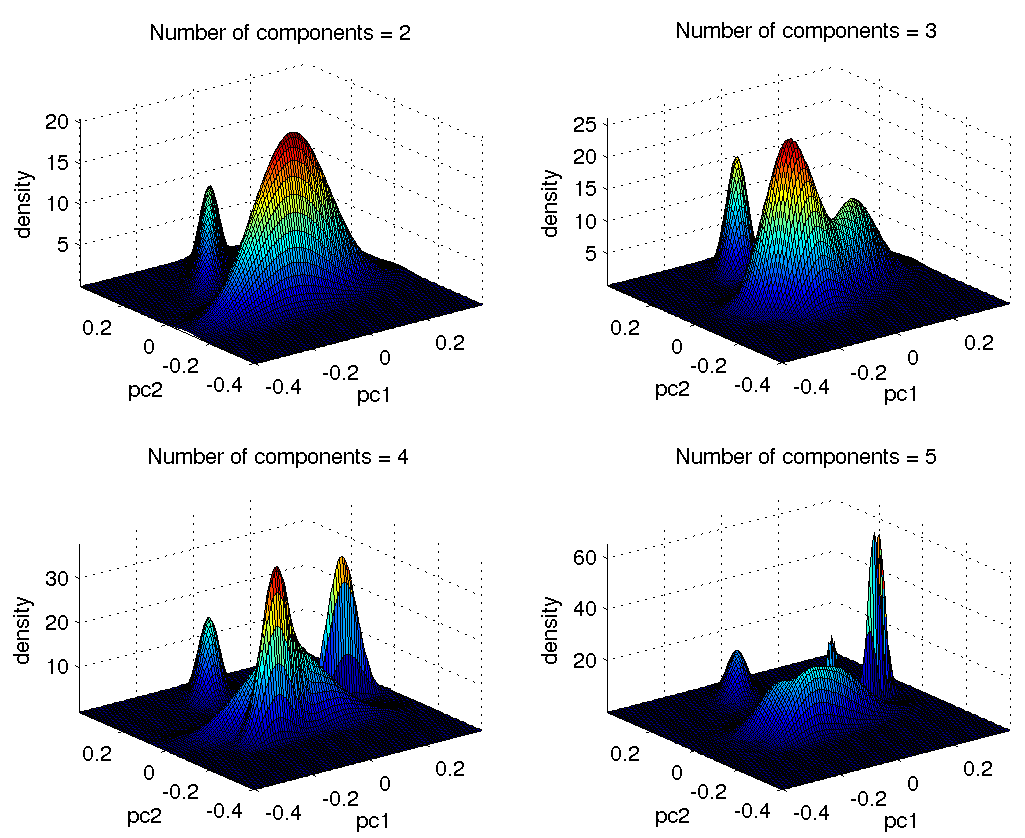
\includegraphics[width=0.95\textwidth]{./images/q37mog}
  \caption{Shows mixtures of gaussians for various selections of
    components in the model.}
  \label{fig:q37mog}
\end{figure}

It is unfortunately not possible to run \emph{gmdistribution.fit}
without specifying the number of components one wants to use within
the model. Thus, it cannot be configured to automatically figure out what
number of components to use. We can instead try to use Akaike
Information Criterion for the estimated models, this idea is good
enough in theory. But as it turns out, it will always favor the one
with the largest number of components, even though this will be
severely over-fitted. As it turn out, if we let it run through
$1$--$11$ components, it will select $11$ and this is with the AIC
value: $-237.657405$, this is based on minimizing a negative log
likelihood function (More information can be found by searching for
\emph{aic} within the Matlab help system). A figure of the 'best'
number of components can be seen in figure \ref{fig:q37mogbest}, where it is
very apparent that the model has collapsed onto a data point as it
peaks around $500$. And when selecting more that $11$ components, the
programs breaks down with the following error: \emph{Ill-conditioned
  covariance error occurred in every replicate.}

\begin{figure}[!htbp]
  \centering
  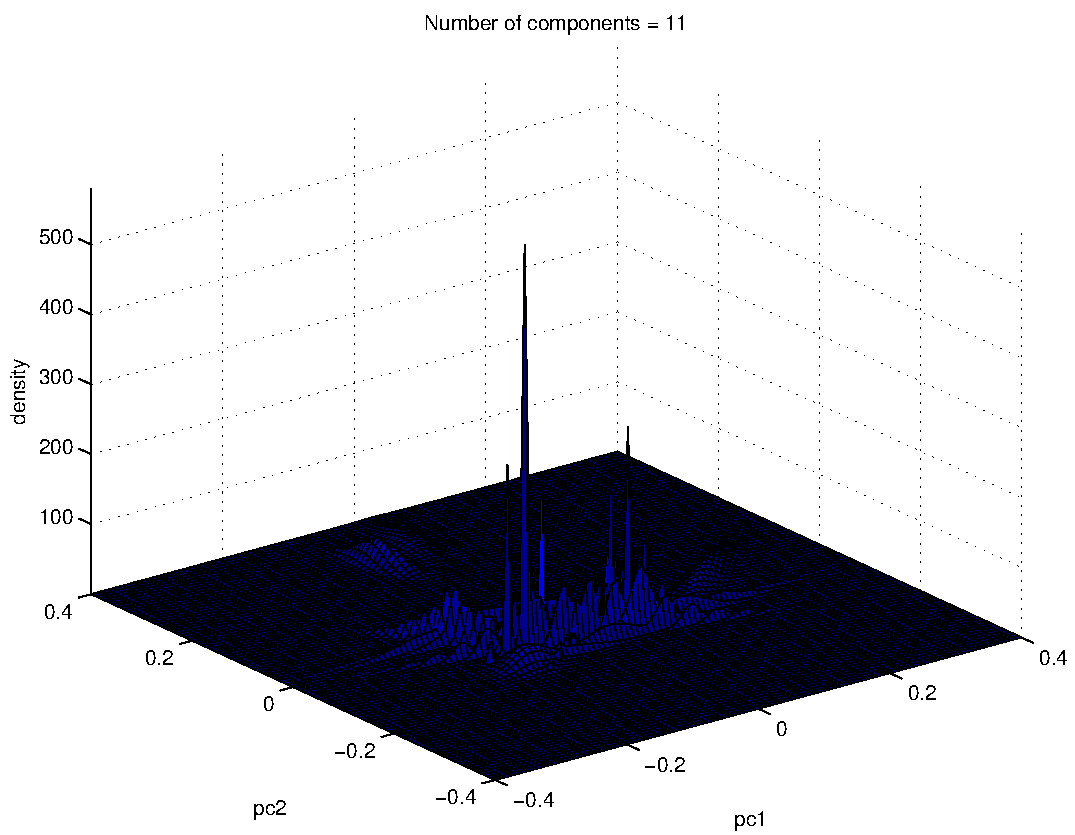
\includegraphics[width=0.95\textwidth]{./images/q37mogbest}
  \caption{Shows the 'best' mixtures of gaussians model.}
  \label{fig:q37mogbest}
\end{figure}
